%%
%% Dit is het hoofddocument: compileer dit met latex of xelatex en je krijgt de gehele pdf
%%
\documentclass[a4paper,11pt,final]{article}
%
%% option = draft will generate black except with \color, replace images by a rectangle
%% option = final will generate color
%

\usepackage{color}
\usepackage[all]{nowidow}
\usepackage{bold-extra}
\usepackage{footmisc}% granting the ability to use label for a footnote
\usepackage{subfig}
\usepackage{wrapfig}% product wrapfigure and wraptable
\usepackage{array}% additions to tabular
%\usepackage{supertabular}% multiple pages tabular
\usepackage{longtable}% multiple pages table like tabular
\usepackage{rotating}% for the environment sidewaysfigure / sidewaystable
\usepackage[english]{babel}
\usepackage{graphicx}
\usepackage{url}
\usepackage{hyperref}% Load after biblatex
\hypersetup{
    colorlinks = true,
    citecolor = blue,
    linkcolor = blue
}
\usepackage[prependcaption,colorinlistoftodos,obeyFinal,textsize=tiny]{todonotes}% when generating final (documentclass option) skip notes
\usepackage{pdflscape}
\usepackage[a4paper]{geometry}
\usepackage{titlesec}% added to change section headers, see newcommand definition.
\usepackage{boxedminipage}
\usepackage{amssymb}% For \checkmark
\usepackage{pifont}% for \ding{'-code or "-code}
\usepackage{listings}

\bibliographystyle{plain}% unsrt, plain, alpha, abbrv

\newcommand{\biburl}[1]{\hspace*{\fill}\\\url{#1} accessed oct/nov 2014}

\author{ABI team 33\\
		Guus Bonnema, Stefan Versluys en Jeroen Kleijn
		}
\date{22/04/2015}

\title{\color{blue}System documentation}

\setlength\extrarowheight{2pt}% Adds a little space at the top of table rows

%% Document is in subdocumenten gesplitst.

\begin{document}

\selectlanguage{english}
\hyphenation{func-tio-nal}

\nowidow% needs package nowidow

%%%%%%%%%%%%%%%%%%%%%%%%%%%%%%%%%%%%
\newcommand{\xmas}{x\textsc{mas}}%
\newcommand{\ok}{$\checkmark$}
\newcommand{\w}[1]{\textbf{\textsc{#1}}}
\newcommand\bw[1]{{\color{blue}#1}}

\newcommand{\mybox}[1]{\begin{boxedminipage}[t]{\textwidth}#1\end{boxedminipage}}

%\definecolor{airforceblue}{rgb}{0.36, 0.54, 0.66}%%   This is color in hex #5D8AA8

%%%%%%%%%%%%%%%%%%%%%%%%%%%%%%%%%%%% different section format start %%%%%%%%%%%%%%%%%%%%%%%%%%%%%%%%%
%\newcommand\secformat[1]{%
%    {\fontsize{60}{60}\selectfont\thesection}%
%    \ifthenelse{\equal{\thesection}{}}{}{\quad\rule[-8pt]{2pt}{40pt}\quad}
%    \parbox[b]{.7\textwidth}{\filright\bfseries #1}}%
%\titleformat{\section}[block]
%    {\filright\normalfont\sffamily}{}{0pt}{\secformat}
%\titlespacing*{\section}{0pt}{*3}{*2}[1pc]
%%%%%%%%%%%%%%%%%%%%%%%%%%%%%%%%%%%% different section format end   %%%%%%%%%%%%%%%%%%%%%%%%%%%%%%%%%

\newcommand\smp[1]{%
	\marginpar{\color{blue}\small\bf\textsc#1}
}%
\newcommand\smpp[1]{\smp{#1}#1}


\maketitle

\begin{abstract}

This document contains the system documentation for the xMAS Model Designer.
It describes the design and implementation details of the designer, the integration with
verification tools, changes to existing code and techniques used for the implementation.

\end{abstract}

%\listoftodos   %% commented out when creating final document
%\tableofcontents

\section{Story tree}

Stories of the xMAS model designer project can be found in the Agilefant data in the xMAS repository.
To use this data you must set up Agilefant on a web server and import xmas/6-transition/08-agilefant/Agilefant_xMAS.zip

The stories are based on three roles:
\begin{itemize}
\item A \textbf{researcher} develop formal verification methods to test on xMAS models.
\item A \textbf{designer} create and verify xMAS models with the xMAS model designer toolkit. 
\item A \textbf{maintainer} that maintains the xMAS model designer toolkit project. 
\end{itemize}

Figure~\ref{fig:story-tree} is a small copy of how this story tree looks like in the Agilefant tool.


\begin{figure}[here]
\begin{center}	
	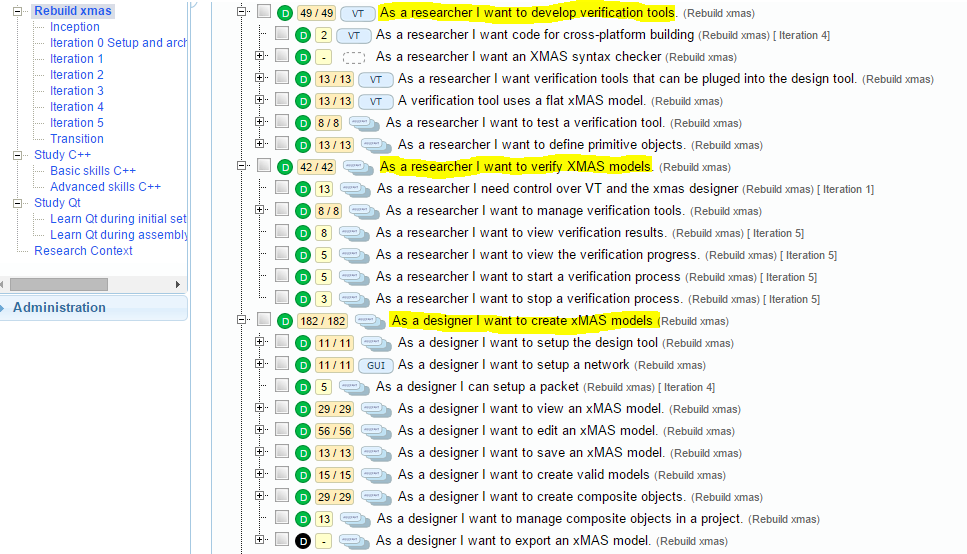
\includegraphics[width=.70\linewidth]{pictures/story-tree}
	\caption{Agilefant story tree}
	\label{fig:story-tree}
\end{center}
\end{figure}


\section{Changes to the data model}

Due to requirements imposed by the designer, several changes and additions have
been made to the data model. Most of these changes are related to the additional
support for hierarchical networks in the designer. This section present an overview
of new and modified classes and functions.

\subsection{XMASNetwork}

XMASNetwork is a new class designed to represent an xMAS network. This class can be
used to model both flat and hierarchical networks. When used to model hierarchical
networks, an XMASNetwork represents a single level or subnetwork in the hierarchy.
Multiple networks are combined to form the complete network.

The main responsibility of XMASNetwork is to serve as a container of XMASComponent
instances. Internally, XMASNetwork stores the components in a map relating a
components name to its in-memory instance. Prior to the introduction of XMASNetwork,
the concept of an xMAS network was directly represented by such a map. Verification
tools still use this approach, although they could be easily adapted to use
XMASNetwork as well.

\paragraph{}
The 'promotion' of XMASNetwork to its own class definition has two primary reasons:
\begin{itemize}
 \item The designer uses additional network properties like the canvas size. These
 properties must be stored somewhere in the data model (i.e. in XMASNetwork).
 \item Support for hierarchical networks requires management of multiple network
 models. Using an explicit class to represent networks eases this task.
\end{itemize}

\paragraph{Extending networks}
XMASNetwork implements the same extension mechansism as used by the XMASComponent and
Port classes. For this, a new class named XMASNetworkExtension has been created.
Currently, the designer uses two network extensions. One to store network
properties common to all models, and one to store network properties specifically
for network models that are to be used as composite objects.
In the future, additional network extensions could be defined, for example to store
data required to support parameterization of subnetworks.

\paragraph{MemoryPool}
All components in an XMASNetwork are stored in a MemoryPool for optimal performance.
Multiple networks can share a MemoryPool instance. The XMASNetwork constructors
optionally take a pointer to a MemoryPool. Passing the same instance to multiple
networks will let these networks share the pool. When no MemoryPool pointer (or
nullptr) is provided to the constructor, XMASNetwork will create its own
MemoryPool instance. In this case, XMASNetwork also takes care of the MemoryPool
destruction.


\subsection{XMASComposite}

When modelling a hierarchical network, composite objects are used to represent
subnetworks as black boxes inside a higher-level network. The addition of
composite objects to an xMAS network is reflected in the data model through the
new XMASComposite class. Like the eight xMAS primitive types, XMASComposite
is derived from XMASComponent. As such, XMASComposites can be used in the same
way as the primitive components.

When a new XMASComposite object is created, a reference to an XMASNetwork must
be passed to the constructor. The composite object will represent an
instantiation of this (sub)network.

The sinks and sources of the subnetwork are used as interface ports or gates
between the subnetwork and the higher-level network. An xMAS source component
will result in an Input port on the composite object. Likewise, each xMAS sink
component in the subnetwork leads to an Output port on the composite object.

\subsubsection{Hierarchical visitors}

Due to the introduction of the new XMASComposite type, the XMASComponentVisitor
interface has been extended to support composite objects. Unlike the existing
pure virtual visit functions, XMASComponentVisitor provides a default
implementation to visit XMASComposites. This way, exisiting implementations of
the interface which weren't designed to support composites aren't affected. The
default visit implementation for composite objects does throw an Exception however.
So, only flat, composite free networks should be passed to these implementations.


\subsection{XMASProject}

The xMAS designer application uses the XMASProject class to manage a complete
hierarchical model. The root network, available through getRootNetwork(), is
the network under construction. For each composite object type used, XMASProject
additionally stores its network definition. XMASProject is equipped with member
functions to insert new components into the network, remove them from the network
and change the name of a component. All of these functions act upon the root network.
Adding a new composite object to the model requires that its network definition
is added to the project in advance. Function insertComposite() automatically does
this if necessary. A subnetwork that is no longer of use can be unloaded using
unloadNetwork(). Unloading only succeeds if no composite objects in the project
(at any level) depend on the network.

XMASProject is also responsible for the construction and destruction of a MemoryPool.
All networks loaded in the project share this instance of the pool.

\paragraph{Note:}
Currently, the designer assumes that all subnetworks used in a project are
stored in the same directory as the root network.


\subsection{Parser \& Exporter}

The additional support for hierarchical models and the need to store data used
by the designer require a number of modifications to the parser and the exporter.

\paragraph{Position}
For each component listed in the json data, the parser checks whether canvas data
is available in the pos field (see also the file format description). If this is
indeed the case, the x, y, orientation and scale fields are read and stored inside
an extension of the component (CanvasComponentExtension). If no position data
is stored in the json data, the designer will use default values. The exporter has
been updated to write the positition data, if present, back to json as well.

\paragraph{Composite objects}
XMASComposite objects are created for all components in the json file with type
'composite'. The parser uses the 'subnetwork' attribute mandatory for composite
components to determine what kind of composite object should be created. The
parser is not responsible for loading subnetworks. Rather, the caller of the parser
must suply a function that is able to map a subnetwork name to an instance of
an XMASNetwork. Code that uses the parser should be updated to comply with the
new function signature. The implementation in XMASProject can be used as a reference.




\subsection{Flattening the network}

\subsection{Changes to the xmas file format}

\section{Feedback interface (not data model related, move to other file?)}

\newpage

% include forces page break. Input does not.
\section{XMD - XMV integration}

\subsection{QML / C++ integration}

\subsubsection{Context property}

\begin{figure}
    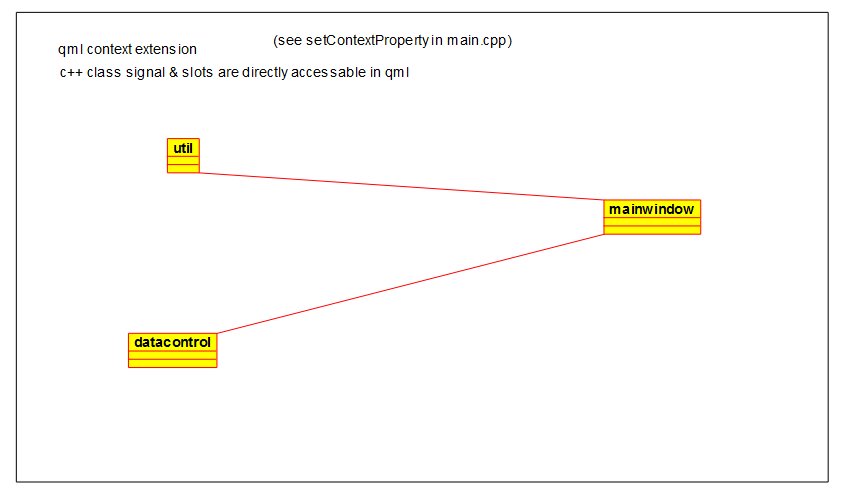
\includegraphics[width=\textwidth]{qml-context-property}
    \caption{Qml / C++ integration using a context property}
\end{figure}


\subsubsection{C++ extension class}

\begin{figure}
    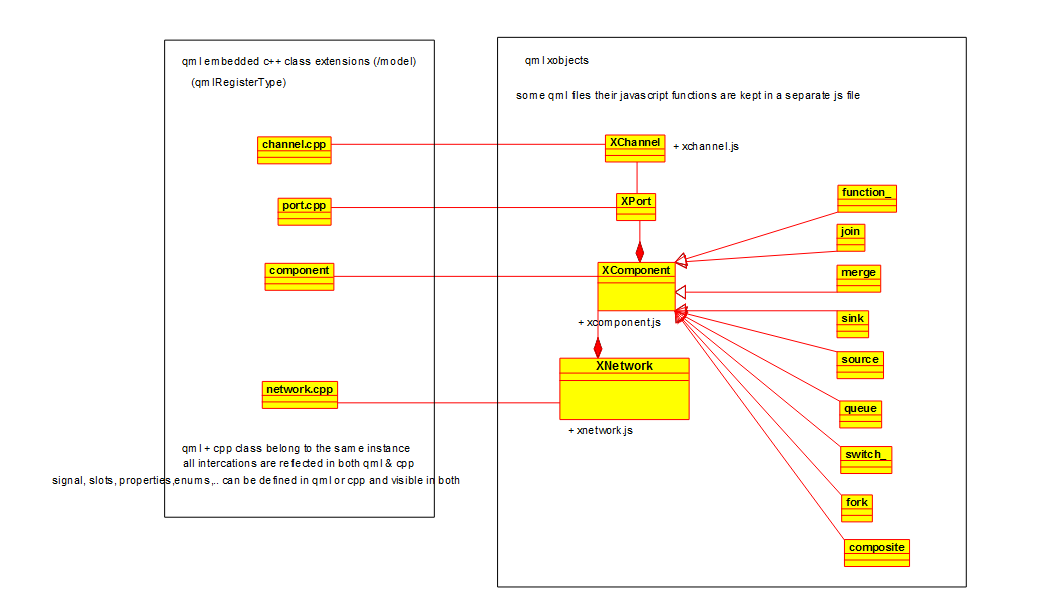
\includegraphics[width=\textwidth]{qml-cpp-extension}
    \caption{Qml/ C++ integration using an extension class}
\end{figure}


\subsubsection{Interaction xmd / datamodel classes}

\begin{figure}
    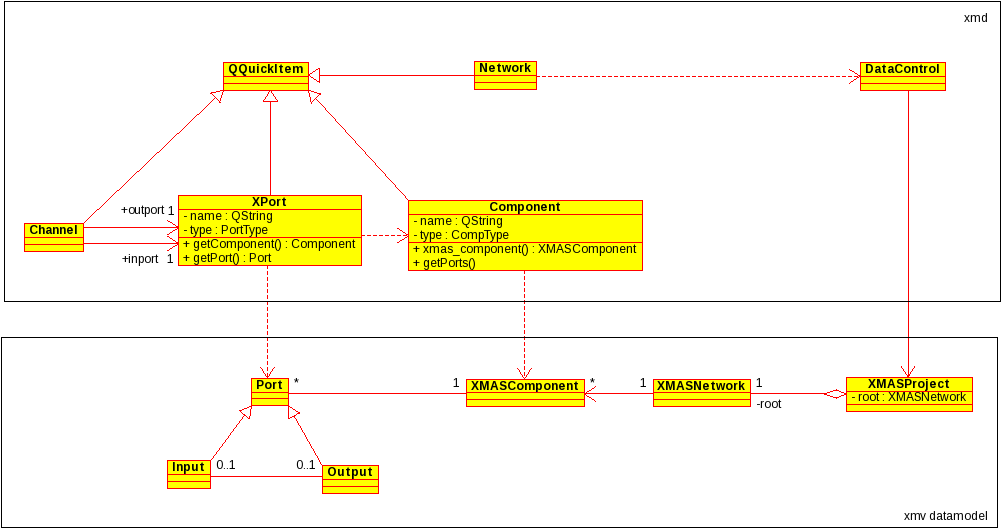
\includegraphics[width=\textwidth]{xmd-xmv-integration}
    \caption{Integration of xmd and xmv datamodel}
\end{figure}

\section{Flattening the network}

Hierarchical networks are flattened before they are processed by the verification
tools. Flattening produces a new flat network, the original network is not modified.
The algorithm broadly consists of the following three steps:
\begin{enumerate}
 \item Copy the components from the hierarchical network to the flat network.
 \begin{itemize}
  \item For composite objects, the flattener instantiates a copy of the subnetwork
  into the target network. Through recursion of the flattening algorithm, this
  subnetwork is first flattened itself.
 \end{itemize}
 \item Connect the channels between the components in the flat network.
 \item Connect all (flattened) subnetworks
\end{enumerate}


\subsection{Algorithm}
The flattening process uses a recursive algorithm to flatten all composite objects.
Each recursive call takes two parameters: the destination network, which is the same
in all recursive calls, and the source network. In each recursion step, a flat copy
of the source network is inserted into the destination network. The projects root
network is the source network in the first iteration. In subsequent recursion steps,
the subnetworks that define a composite object are used as source networks.

\paragraph{Gates}
In a subnetwork, sources and sinks are used to define the interface between the
subnetwork and the higher-level network. In the flattened network these components
are no longer present. Components in the higher-level network are directly connected
to the components in the subnetwork. Alternatively, when there is a channel between two
composite objects, the components of two subnetworks directly connect to each other.
To prepare for connection of the networks, sources and sinks are replaced during
flattening by temporary components called gates. An XMASSource component gets replaced
by an XMASInGate component. This component has an additional Input port (i\_ext) that
corresponds to the Input port of the composite object in the higher-level network.
Likewise, an XMASSource is converted to an XMASOutGate instance, which has an
additional Output port (o\_ext). Figure~\ref{fig:mc-gates} shows the result.

\begin{figure}[ht]
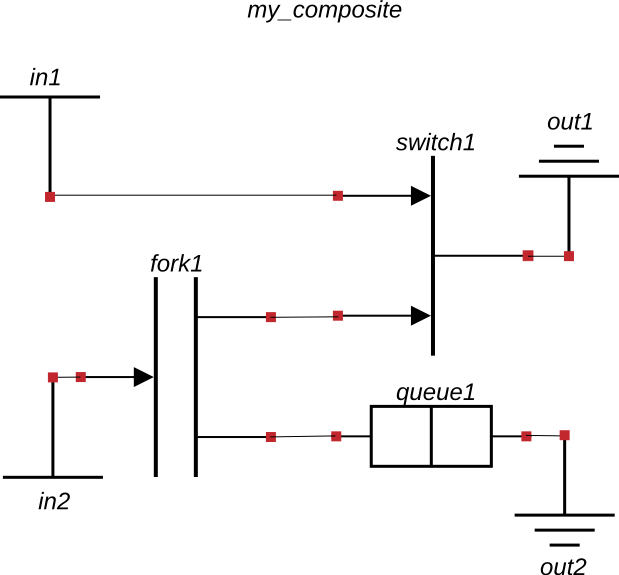
\includegraphics[width=0.4\textwidth]{my_composite-network}
\hfill
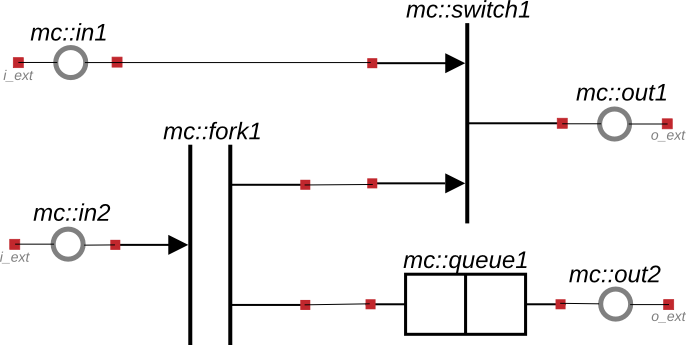
\includegraphics[width=0.5\textwidth]{my_composite-gates}
  \caption{The original composite network (left) and a partial view of the flattened
  network showing the subnetwork with gates (right); the component names have been
  qualified with the composite objects name (mc) to prevent name collisions}
  \label{fig:mc-gates}
\end{figure}


\paragraph{Flattened composite}
The result of a recursion step is a flattened subnetwork. Moreover, the recursion
step generates a number of gates which are still not connected to the external
world. Upon return of a recursive call, these gates are collected and stored in
another temporary component: XMASFlattenedComposite. This component is the direct
equivalent of an XMASComposite in the source network.

\paragraph{Connecting channels}
The second step, connecting the channels between components is easy. Although
composite objects are flattened, the temporary XMASFlattenedComposite objects
are still present. They provide the same interface (Input and Output ports) as
the XMASComposite object in the source network. Connecting to a composite is a
matter of connecting channels to the external ports available on the
XMASFlattenedComposite instances. Even self-connecting composite objects can be
handled this way. Figure~\ref{fig:flattened-composite} details the preceding
two steps.

\begin{figure}[ht]
    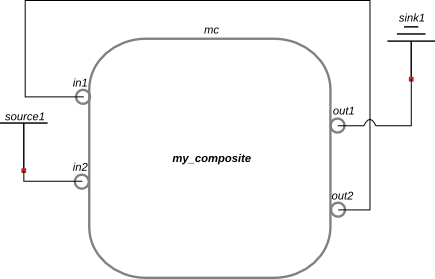
\includegraphics[width=0.5\textwidth]{example-hier-network}
    \hfill
    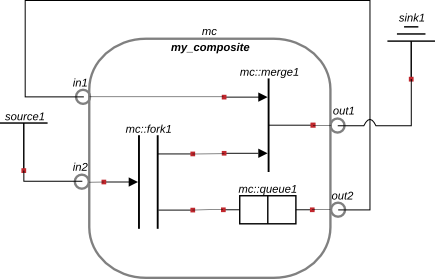
\includegraphics[width=0.5\textwidth]{example-hier-network-inserted}
    \caption{The root network (left) containing a composite object and the
    corresponding flattened network (right) including the XMASFlattenedComposite object}
    \label{fig:flattened-composite}
\end{figure}

\paragraph{Cleaning up}
The final step, per recursion, is to remove the temporary components and gates.
For each flattened composite, all gates are iteratively removed by simply
updating both ports on the opposite ends of the gates ports so that they
directly connect to each other. After this, the XMASFlattenedComposite and its
gates are deleted.


\begin{figure}[ht]
    \centering
    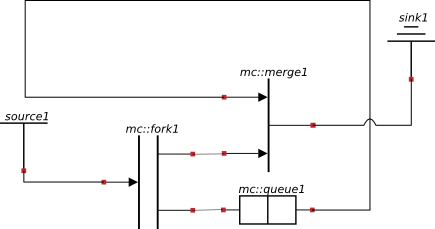
\includegraphics[width=0.5\textwidth]{example-hier-network-final}
    \caption{The resulting flattened network}
    \label{fig:final-network}
\end{figure}




%\paragraph{Gates}
%During flattening of a subnetwork, XMASSources and XMASSinks that represent the
%interfaces of a subnetwork are converted to gates. An XMASSource becomes an
%XMASInGate and an XMASSink becomes an XMASOutGate. Gates are similar to sources
%and sinks but they have an additional port that will be used to connect the gate
%to the external, higher-level network.




%Each recursive call will only create primitives in the destination network. At
%the deepest recursion level, for which the subnetwork contains no composite objects,
%this is simply a matter of copying the primitives*. After the subnetwork has been
%instantiated, one or more interface ports

%Additionally, temporary objects are created to the 

%The flatten function returns a list of all connection points called gates. These
%gates correspond to the sources and sinks in the (sub)network. The 


%The flattening algorithm uses three auxiliary component classes: XMASInGate, XMASOutGate
%and XMASFlattenedComposite. Temporary instances of these classes are created to
%bridge the gap between a subnetwork and the network that contains the composite object.

%* Parameterization of the network!
%Value parameterization: e.g. using a credit-counter with 12 tokens and a credit-counter
%with 5 tokens.

%Structural parameterization: e.g. mesh, spidergon (see proposal)

%\paragraph{XMASFlattenedComposite}
%The actual flattening a composite 
%When a subnetwork has been 
%From the higher-level networks perspective, composites 





%The gates are
%used as interfaces between a subnetwork and the higher-level network. An XMASSource
%component that acts as an input 
%The actual flattening occurs in steps 1 and 3. 

\paragraph{Note:}
While copying a component, all known extensions that a component can have are
copied as well. Which extensions to copy for what component type is currently
hard-coded in the flattener. Ideally, this method will be replaced by a more
generic copying method. Its implementation has been postponed due to changes
required to the underlying bitpowder library. 




\section{Feedback interface}

While analyzing a network, verification tools can generate various types of
feedback messages. At this moment, verification tools present this feedback
as human readable text messages on the standard output. Although this form
is suitable for human consumption when running the verification tools as a
standalone application, they are hard to parse and interpret by software like
the designer.

Due to time constraints, presentation of feedback from the verification
tools has been kept simple. Similar to the standalone application, the
text messages are presented to the user in a text console integrated in
the designer. Future improvements could enhance the integration between
designer and verifications. As an example, problematic components and ports
could be highlighted on the design canvas.

\paragraph{}
To support these kinds of enhancements, a more structured way to pass feedback
from verification tools must be used. For this purpose, a feedback message
format has been defined along with several functions that can be used 
by verification tools to generate feedback messages.


\subsection{Message format}
Feedback messages are structured as follows:

\paragraph{}
[\textbf{sender}] **\textbf{type}**: \textbf{message}
(\textbf{component list}) (\textbf{port list})


\begin{itemize}
    \item \textbf{sender} is a string to identify the verification tool that
    sends the feedback message. Each verification tool should define a unique
    name to identify itself.
    
    \item \textbf{type} specifies the type of feedback. The following feedback
    types are defined:
    \begin{itemize}
        \item \textbf{INFO} - informational message, e.g. verification tool has started or finished
        \item \textbf{WARNING} - non-fatal warning, e.g. non-optimal network configuration detected
        \item \textbf{FAULT} - fault in the network detected, e.g. a combinatorial cycle
        \item \textbf{CRASH} - crash / unexpected exception thrown by the verification tool,
        this indicates a programming error, not a network fault
        \item \textbf{PROGRESS} - informational message containing progress of a verification tool
    \end{itemize}

    \item \textbf{message} contains the actual feedback message. Verification tools can pass
    custom text messages. For PROGRESS type feedback, the message field has a fixed format:
    ``progress/total'' where both progress and total are positive integers.
    
    \item \textbf{component list} is an optional list of component IDs to which the feedback
    applies. The components are listed inside brackets using comma-separated notation and are
    prefixed by ``Comp: '', e.g. Comp: [src1, join2, ...].

    \item \textbf{port list} is an optional list of ports (of components) to which the feedback
    applies. The ports are listed inside brackets using comma-separated notation and are
    prefixed by ``Port: '', e.g. Port: [src1.o, join2.a, ...].
    
    \item messages are terminated by a newline character
    
\end{itemize}


\subsection{Example}

\begin{verbatim}
[cycle-checker] **INFO**: Starting cycle checker
[cycle-checker] **FAULT**: Combinatorial cycle detected!  Port: [::frk0.a]
[cycle-checker] **INFO**: Finished! 
\end{verbatim}


\subsection{Current state \& future work}

The ``cycle checker'' verification tool has been adapted to output its feedback in the
described format. Optionally, this tool could be updated to emit progress information.
However, progress information is of little value due to the short runtime of this tool.

As mentioned earlier, the designer does not interpret the feedback message structure yet.
Extracting the information from the text string can be accomplished through the use of a
regular expression. All feedback formatting code is located in the feedback-interface.h/cpp
files. Changes to the message format and new code to parse the message string can be added
here.
\section{XMAS network file format}\label{xmas-network-file-format}

This document describes the file format used to store XMAS network
models. Both the XMAS designer application and the standalone
verification tools use this file format. The structure is based on the
flat json format used by the checker application provided at the start
of this project. Several new fields have been added in order to support
hierarchical networks and information specific to the designer. As the
new file format is able to support both flat and hierarchical networks,
the (recommended) file extension has been changed from fjson to json.

\subsection{Root JSON object}\label{root-json-object}

Properties:

\begin{itemize}
\itemsep1pt\parskip0pt\parsep0pt
\item
  ``CANVAS'' : the \textsc{Canvas} object (optional) \emph{NEW}
\item
  ``COMPOSITE\_NETWORK'' : the \textsc{Composite\_Network} object (optional)
  \emph{NEW}
\item
  ``VARS'' : the \textsc{Vars} object
\item
  ``PACKET\_TYPE'' : the \textsc{Packet\_Type} object
\item
  ``NETWORK'' : an array of \textsc{Component} describes all components in
  the network
\end{itemize}

\subsection{CANVAS}\label{canvas}

\textbf{\emph{NEW}} Used by the XMAS designer application to define
properties of the designer canvas. When no \textsc{Canvas} information is
specified, default values are used.

Properties:

\begin{itemize}
\itemsep1pt\parskip0pt\parsep0pt
\item
  ``width'' : width of the canvas in logical units
\item
  ``height'' : height of the canvas in logical units
\end{itemize}

\subsection{COMPOSITE\_NETWORK}\label{compositeux5fnetwork}

\textbf{\emph{NEW}} Contains designer specific information to use this
network as a composite object. If this information is not present, the
network cannot be used as a composite object.

Properties:

\begin{itemize}
\itemsep1pt\parskip0pt\parsep0pt
\item
  ``alias'' : displayed inside a composite object to denote the objects
  type (e.g.~mesh)
\item
  ``image-name'' : name of graphical resource used as a symbol to denote
  the objects type (e.g.~mesh.ico)
\item
  ``boxed-image'' : set to 1 to use the image as a symbol inside a
  generic composite object (drawn boxed) or set to 0 to use the image as
  the graphical representation of the entire component, this can be used
  to draw common macro's like credit counters and delays using the
  symbols commonly used in literature to denote these macro's.
\item
  ``packet'' : The verification system does not use this information yet, 
  				although the user interface does allow entering a value.
  				Its value is reserved for later use.
\end{itemize}

\subsection{VARS}\label{vars}

\emph{TODO}\footnote{\label{fileformat-todo}The semantics of this field 
were not changed from the original file format.
It is up to the customer to define the contents of this field.}
Definition taken from original file format.

\subsection{PACKET\_TYPE}\label{packettype}

\emph{TODO}\footref{fileformat-todo}
Definition taken from original file format.

\subsection{COMPONENT}\label{component}

Describes a component in the network.

Properties:

\begin{itemize}
\itemsep1pt\parskip0pt\parsep0pt
\item
  ``id'' : \textsc{String} - unique identifier
\item
  ``type'' : \textsc{Component\_type} enum - type of the component
\item
  ``outs'' : array of \textsc{Out} - describes all connected output
  ports
\item
  ``fields'' : array of \textsc{Field} \emph{(optional)}
\item
  ``pos'' : \textsc{Position} - \emph{new} - position of the component
  on the canvas
\end{itemize}

\subsection{Component\_type}\label{componenttype}

Enumeration:

\begin{itemize}
\itemsep1pt\parskip0pt\parsep0pt
\item
  source
\item
  sink
\item
  function
\item
  queue
\item
  xfork
\item
  join
\item
  xswitch
\item
  merge
\item
  composite \textbf{\emph{NEW}}
\end{itemize}

\subsection{COMPONENT {[}type=``source'',
type=``sink''{]}}\label{component-typesource-typesink}

Properties:

\begin{itemize}
\itemsep1pt\parskip0pt\parsep0pt
\item
  ``required'' : \textbf{Boolean 1/0} - set to 1 when this source/sink
  is an interface port of a composite network that must be connected by
  the higher level network. set to 0 when this is optional.
\end{itemize}

\subsection{COMPONENT
{[}type=``composite''{]}}\label{component-typecomposite}

\textbf{\emph{NEW}}

Properties:

\begin{itemize}
\itemsep1pt\parskip0pt\parsep0pt
\item
  ``subnetwork'' : \textsc{String} - name of the subnetwork
\item
  (``parameters'' : (Not determined yet) - reserved property
  name, to be used in the future to parameterize the network)
\end{itemize}

Description: The subnetwork reference indicates the relative location of
the subnetwork on the filesystem.

E.g. ``mesh.json'' refers to the network defined in ``mesh.json'' in the
same directory as this network and ``spidergon/node.json'' refers to the
network defined in ``node.json'' in the subdirectory ``spidergon''.

Parameterization of composite objects has not been implemented yet. When
implemented, composite objects require an additional field in the
component description to store the parameters. The property name
``parameters'' has been reserved for this purpose.

\emph{Note: Currently the XMAS designer requires that all used composite
networks are defined in the same directory as the root network.}

\subsection{OUT}\label{out}

Description: Describes channels between the components in the network.
For each output port of a component, an \textbf{OUT} object describes to
which input port of which component it is connected.

Properties:

\begin{itemize}
\itemsep1pt\parskip0pt\parsep0pt
\item
  ``id'' : \textsc{String} - reference to the target component
\item
  ``in\_port'' : \textsc{Number} - index of the input port on the target
  component
\end{itemize}

\subsection{FIELD}\label{field}

\emph{TODO}\footref{fileformat-todo}
Definition taken from original file format

\subsection{POSITION}\label{position}

\textbf{\emph{NEW}} Stores positional data of the component on the
canvas.

Properties:

\begin{itemize}
\itemsep1pt\parskip0pt\parsep0pt
\item
  ``x'' : \textsc{Number} - x or horizontal position on the canvas
\item
  ``y'' : \textsc{Number} - y or vertical position on the canvas
\item
  ``orientation'' : \textsc{Number} - orientation of the component,
  measured in degrees clockwise.
\item
  ``scale'' : \textsc{Number} - scale factor of the component
\end{itemize}



% Bibliography ---> need to include
%\bibliography{sd}

\end{document} ;########################### end document ##################################;
